\section{JACK's User Interface}\label{SecUI}

One of the features where JACK distinguishes itself from other program
verification tools is the integration in the IDE Eclipse. This ensures
that the application developer does not have to learn the
peculiarities of a new tool, and that he/she does not have to switch
tools to apply formal verification techniques. Instead, the
integration of JACK in Eclipse provides a seamless integration of
formal methods in the application development process. 

The integration in Eclipse consists of two parts: first there is an
extension of the standard Java view with special JACK-related actions
(checking a specification, calling an (automatic) prover \emph{etc.},
second there is a special JACK view that allows to inspect the
generated proof obligations.

\subsection{Extension of the Java View in Eclipse}

The standard Java view of Eclipse is extended with several
JACK-specific features. Menus are added to set the defaults for the
different specification constructs. Further, there are buttons and
menu-options to \emph{e.g.}\ ``compile'' a JML specification,
\emph{i.e.}\ type check the JML specification and generate proof
obligations, call an automatic prover on all the generated proof
obligations (either Simplify or a especially developed Coq tactic), or
change to the JACK view to inspect the generated proof obligations. 

Checking the JML specification is not done automatically, while
editing the file (as is done for Java); instead the user has to launch
this action explicitly. At the time this interface was developed,
adding such automatic checks required too many changes to the
internals of Eclipse, which were not default available. However, in
the mean time such a features has been developed within the JMLEclipse
project\footnote{See
\texttt{http://jmleclipse.projects.cis.ksu.edu/}.}. This project also
provides syntax highlighting of JML specifications in Eclipse's Java
view. It is future work to integrate this with the JACK tool
(\emph{e.g.}\ the JMLEclipse project does not accept the keywords that
JACK adds to JML. 

When integrating these different features with Eclipse, an important
constraint was the tool's responsiveness. An IDE is supposed to be
used interactively, and the developer should never be forced to wait
long for a result. Proof obligation generation is no problem for this,
but calling an automatic prover on the generated proof obligations can
take a significant amount of time. Therefore, the prover is called in
a non-blocking way, launching a special window that allows to see the
progress of the task.

\subsection{A Proof Obligation Inspection View}

An important feature of JACK is that one can inspect the different
proof obligations that are generated. Moreover, one does not have to
understand the specific specification language of the prover that is
being used; instead the proof obligations can be viewed in a
Java/JML-like syntax (but of course, one can also choose to see the
proof obligations as they are generated for a specific theorem
prover). 

\begin{figure}[t!]
\epsfig{file=screen1.ps,angle=270,width=\textwidth}
\caption{JACK's proof obligation inspection view}\label{FigJackView}
\end{figure}

%\begin{figure}[th!]
%    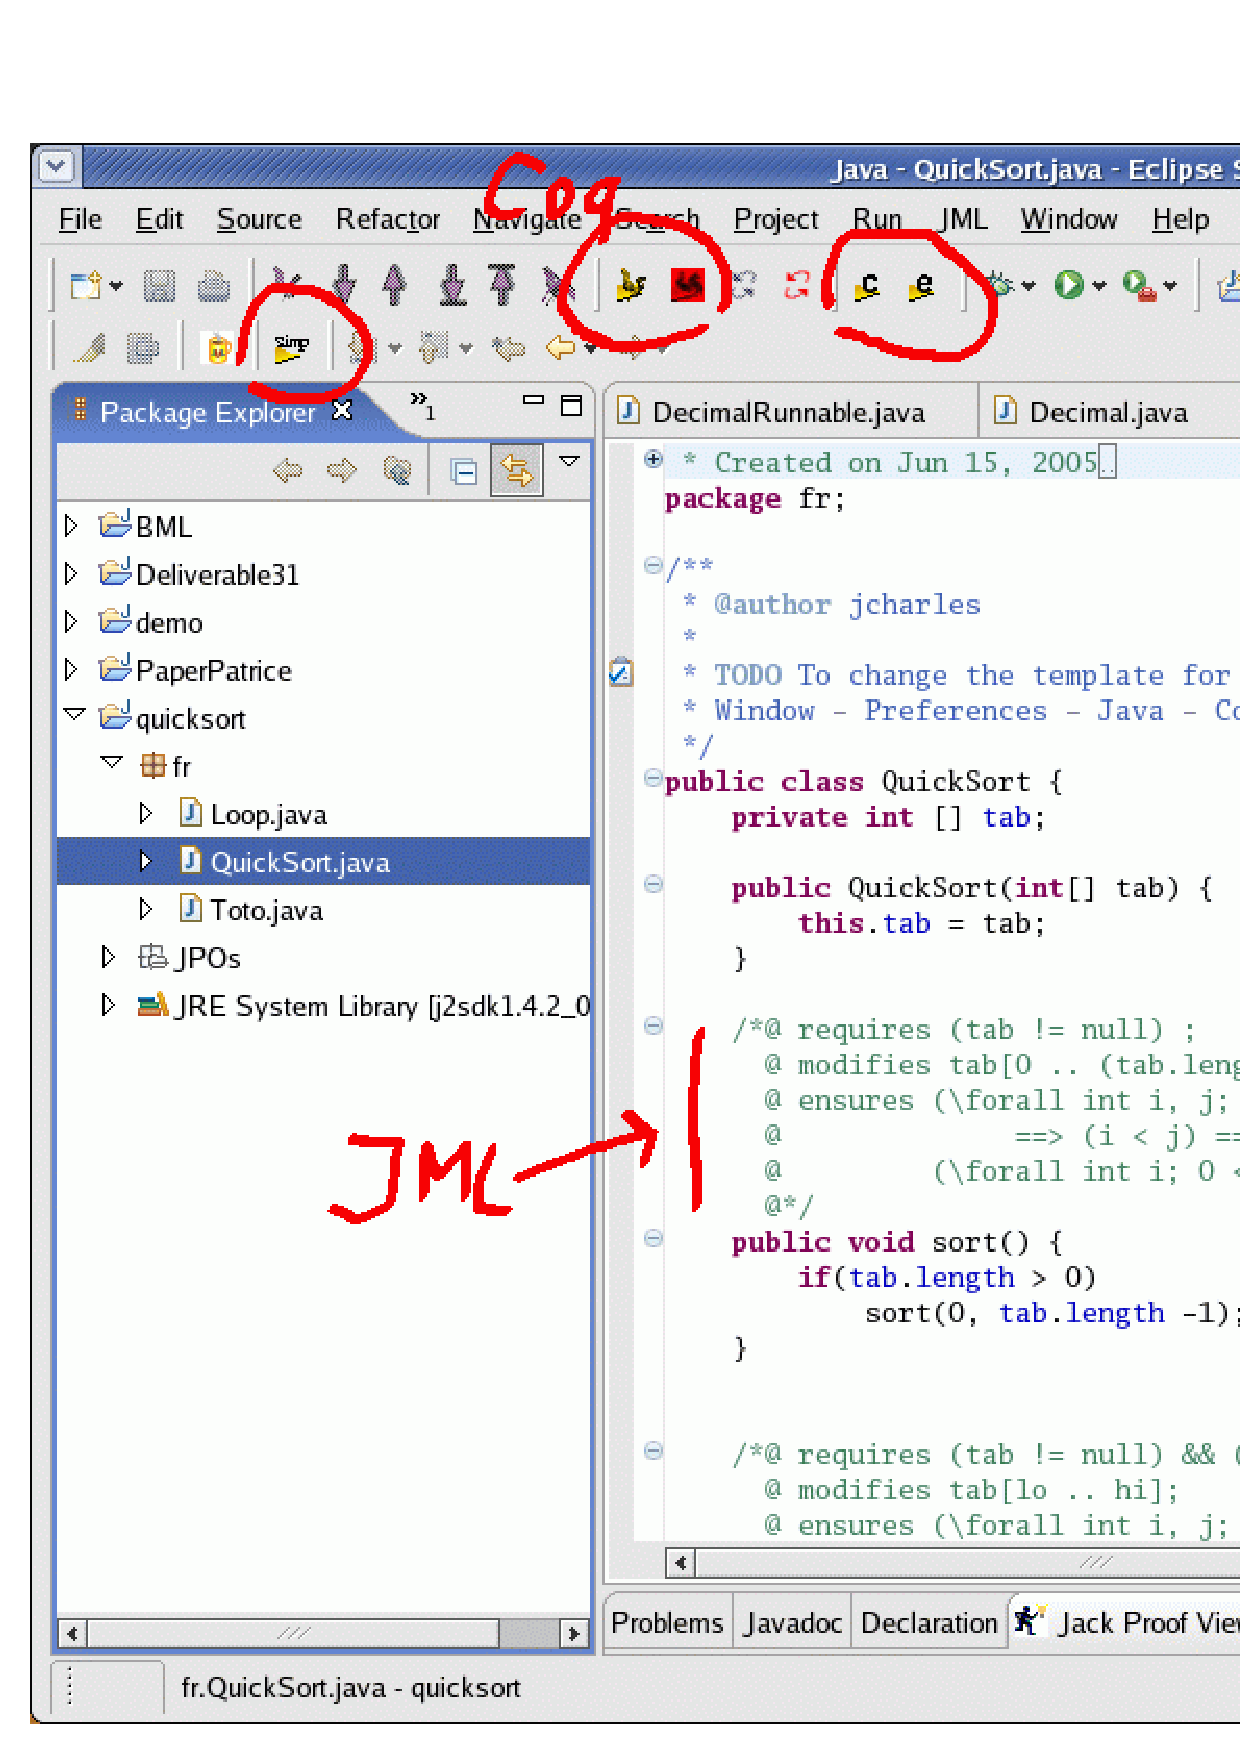
\includegraphics[width=\textwidth]{screen1}
%\caption{JACK's proof obligation inspection view}\label{FigJackView}
%\end{figure}
JACK's proof obligation inspection view provides the following information:
\begin{itemize}
\item information concerning the current proof status;
\item the class methods with their lemmas;
\item the source code; and
\item the currently selected proof obligation (goal and hypotheses).
\end{itemize}
Figure~\ref{FigJackView} shows the inspection of a proof obligation
for the method \texttt{sort} in the QuickSort example of
Figure~\ref{FigJMLSpec}. The left upper windows allows one to browse
the proof obligations for the current class. Proven obligations are
ticked, the others are marked with a cross. The right window shows the
original source code, where the path through the code that corresponds
to the current proof obligation is coloured, together with the
relevant part of the method specification. Different colours have
different meanings: green means normal execution, red means that an
exception is thrown, while blue indicates that additional information
is available (\emph{e.g.}\ whether a condition was true or false).
Moving the mouse pointer over a method name shows the corresponding
method specification, while moving it over blue program text will show
the additional information available. The bottom window shows the
proof obligation: the left half contains the hypotheses, marked with
letters indicating their origin (\emph{e.g.}\ a hypothesis marked R
originates from the methods precondition (requires clause), while a
hypothesis marked L comes from local declarations within the
method. The right half of the window shows the actual goal that has to
be proven. The label of the windows highlights once again that this
proof obligation originates from the postcondition (ensures)
clauses. Finally, notice that the proof obligation is here displayed
in Java syntax, but that buttons are available to change to Coq,
Simplify or PVS syntax.

\marginpar{Say something about 'manual check' option for proof
obligations}

The user can use the proof obligation inspection view to inspect the
different (unproven) proof obligations, and to launch different
(interactive or specialised) provers to prove the remaining proof
obligations.

